% SecondChance -- presentation deck
% Compile on Overleaf. Upload the PNGs from shelter/results/plots/ into a
% folder named "figures" next to this file (or upload the whole shelter folder).
\documentclass[aspectratio=169,11pt]{beamer}

\usetheme{default}
\usecolortheme{seahorse}
\usepackage[T1]{fontenc}
\usepackage{lmodern}
\usepackage{booktabs}
\usepackage{graphicx}
\usepackage{xcolor}

\graphicspath{{figures/}{../results/plots/}{shelter/results/plots/}}

\definecolor{jiitblue}{RGB}{23,54,93}
\definecolor{accent}{RGB}{235,104,52}
\setbeamercolor{frametitle}{fg=jiitblue}
\setbeamercolor{title}{fg=jiitblue}
\setbeamercolor{structure}{fg=jiitblue}
\setbeamertemplate{navigation symbols}{}
\setbeamertemplate{footline}[frame number]
\setbeamerfont{frametitle}{size=\large,series=\bfseries}

\newcommand{\punch}[1]{{\color{accent}\textbf{#1}}}

\title{\textbf{SecondChance}}
\subtitle{Mining attribute bias in animal shelter outcomes}
\author{Sambhav Ghildiyal \and Aniket Pandey \and Aditya Bansal \and Mudit Maheshwari}
\institute{Jaypee Institute of Information Technology, Noida\\
Machine Learning and Data Mining \\ \smallskip
\footnotesize Submitted to Dr. Ashish Mishra}
\date{November 2026}

\begin{document}

\begin{frame}[plain]
  \titlepage
\end{frame}

% ---------------------------------------------------------------- question
\begin{frame}{The question}
  \Large
  Shelters decide, under permanent capacity pressure, which animals get
  promoted, fostered, transferred --- or euthanised.

  \bigskip
  People believe things about what decides an animal's fate.

  \bigskip
  \begin{itemize}\itemsep0.4em
    \item Black animals are passed over
    \item Pit bulls do not get homes
    \item Nobody wants an old dog
  \end{itemize}

  \bigskip
  \punch{These beliefs drive real policy. They are almost never measured.}
\end{frame}

% -------------------------------------------------------------------- data
\begin{frame}{The data}
  \begin{columns}[T]
    \begin{column}{0.56\textwidth}
      Austin Animal Center, public open data.
      \begin{itemize}\itemsep0.35em
        \item 173{,}775 outcome events, Oct 2013 -- May 2025
        \item Joined to 173{,}812 intake events at \punch{99.1\,\%}
        \item 162{,}461 dogs and cats analysed
        \item Two CSVs, no account, no API key
      \end{itemize}
      \bigskip
      Everything is categorical: species, breed, colour, age band, sex,
      intake route, intake condition.
    \end{column}
    \begin{column}{0.42\textwidth}
      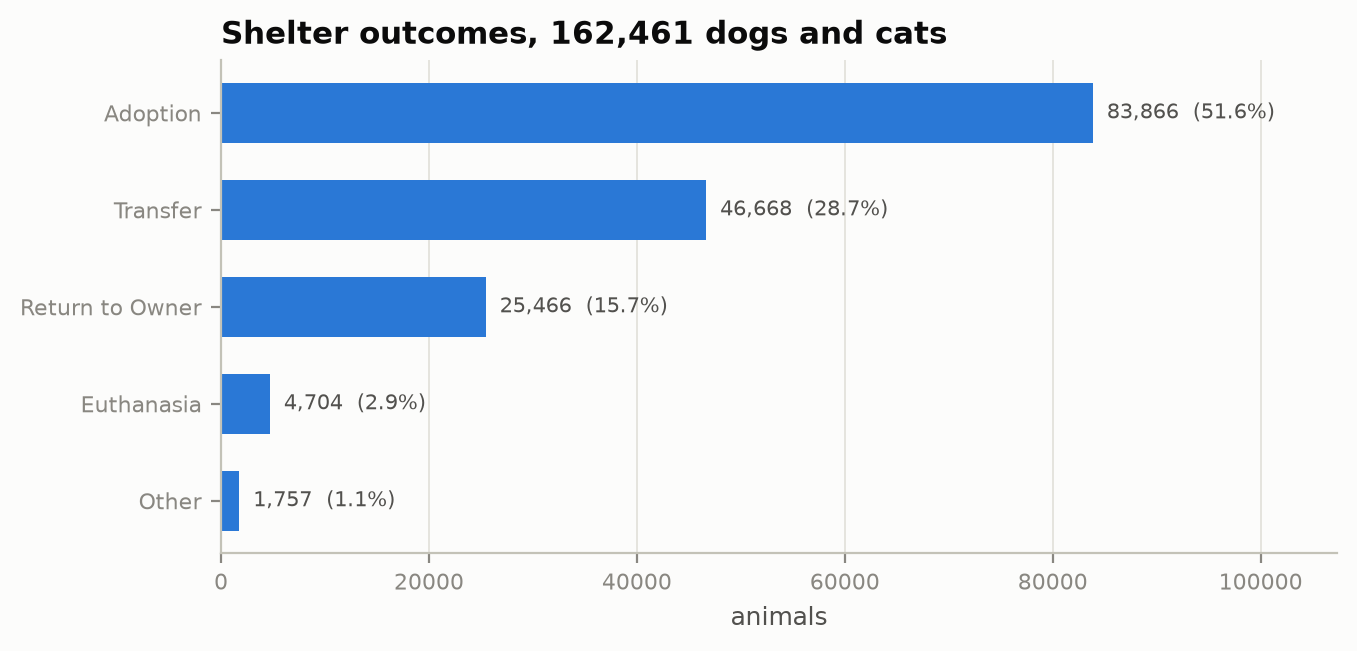
\includegraphics[width=\linewidth]{01-outcomes.png}
    \end{column}
  \end{columns}
\end{frame}

\begin{frame}{Three things that nearly broke it}
  \begin{enumerate}\itemsep0.9em
    \item \textbf{Mixed timezone offsets} in \texttt{DateTime} --- naive and aware
          timestamps cannot be compared. Parse as UTC.
    \item \textbf{10\,\% of animals come back.} The join must be per
          \emph{outcome event}, matched to the most recent prior intake --- not
          one row per animal.
    \item \punch{The obvious feature leaks the label.} \texttt{Sex upon Outcome}
          encodes sterilisation, and shelters sterilise animals \emph{in order to}
          adopt them out. Using it is circular.
          \\[0.2em]
          $\Rightarrow$ every feature comes from the \textbf{intake} record.
  \end{enumerate}
\end{frame}

% ------------------------------------------------------------------ method
\begin{frame}{Method}
  \small
  \begin{tabular}{@{}lll@{}}
    \toprule
    \textbf{Question} & \textbf{Technique} & \textbf{Output} \\
    \midrule
    What goes with what? & Apriori, FP-Growth & rules ranked by lift \\
    What fate can we predict? & Tree, NB, KNN, SVM, MLP & two protocols \\
    What groups exist? & K-Means, K-Medoids, & Hamming \\
                       & Hierarchical, DBSCAN, OPTICS & dissimilarity \\
    Does colour matter? & direct standardisation & like-for-like rates \\
    \bottomrule
  \end{tabular}

  \bigskip
  \textbf{All eleven algorithms from the course. Nothing imported from outside it.}
\end{frame}

% ------------------------------------------------------------------- rules
\begin{frame}{Association rules, ranked by lift}
  \centering
  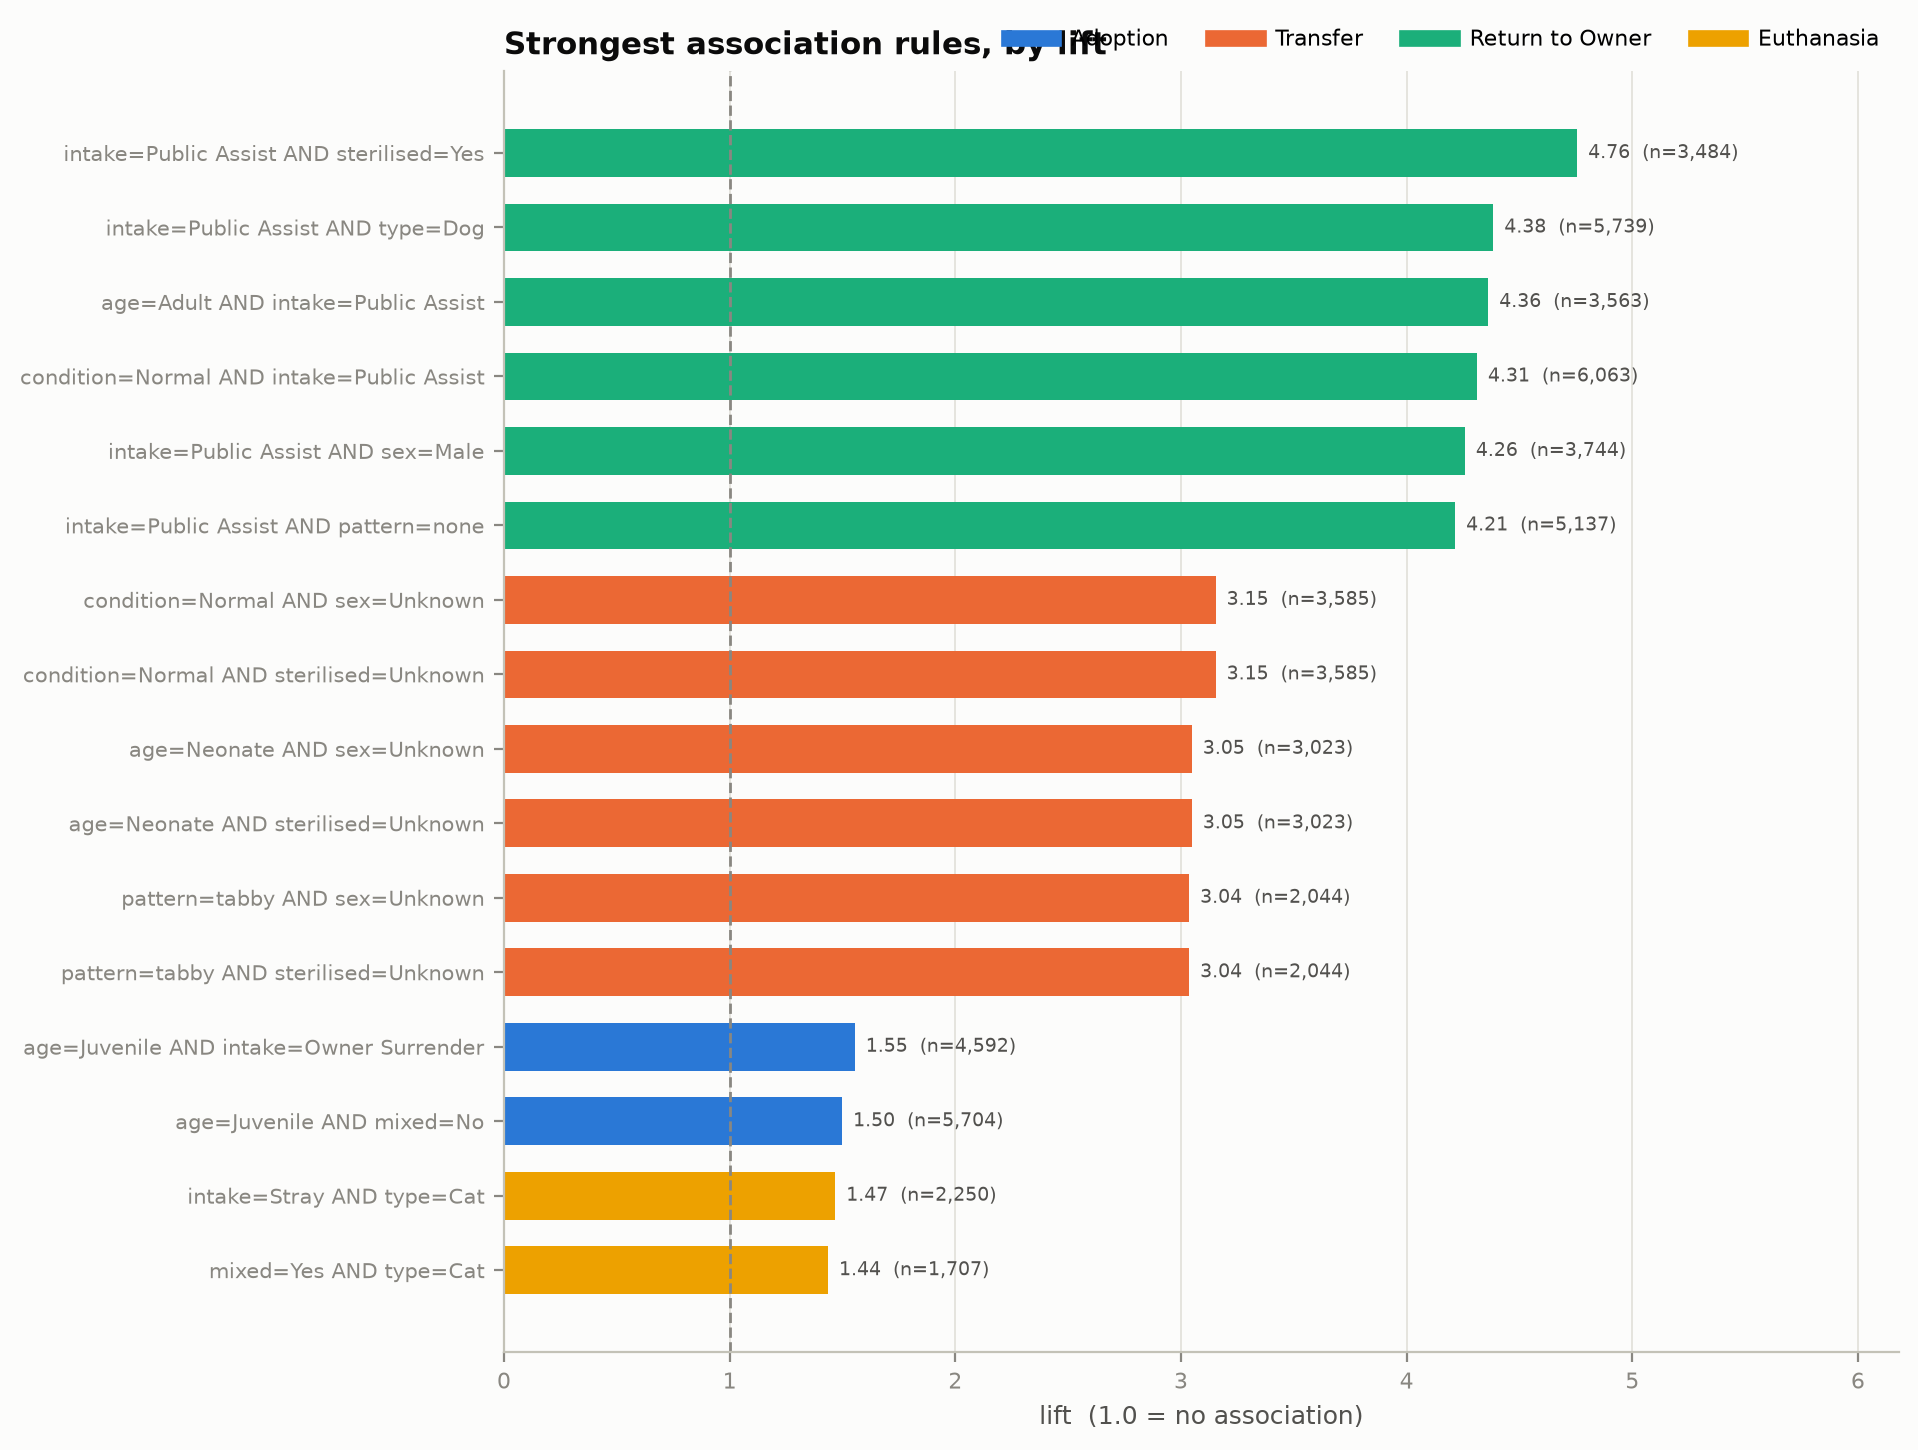
\includegraphics[height=0.72\textheight]{02-rules-lift.png}

  \footnotesize
  Lift, not confidence: Adoption is $\sim$52\,\% of records, so a rule can reach
  0.6 confidence while saying nothing.
\end{frame}

\begin{frame}{Apriori has a price, and you can see it}
  \centering
  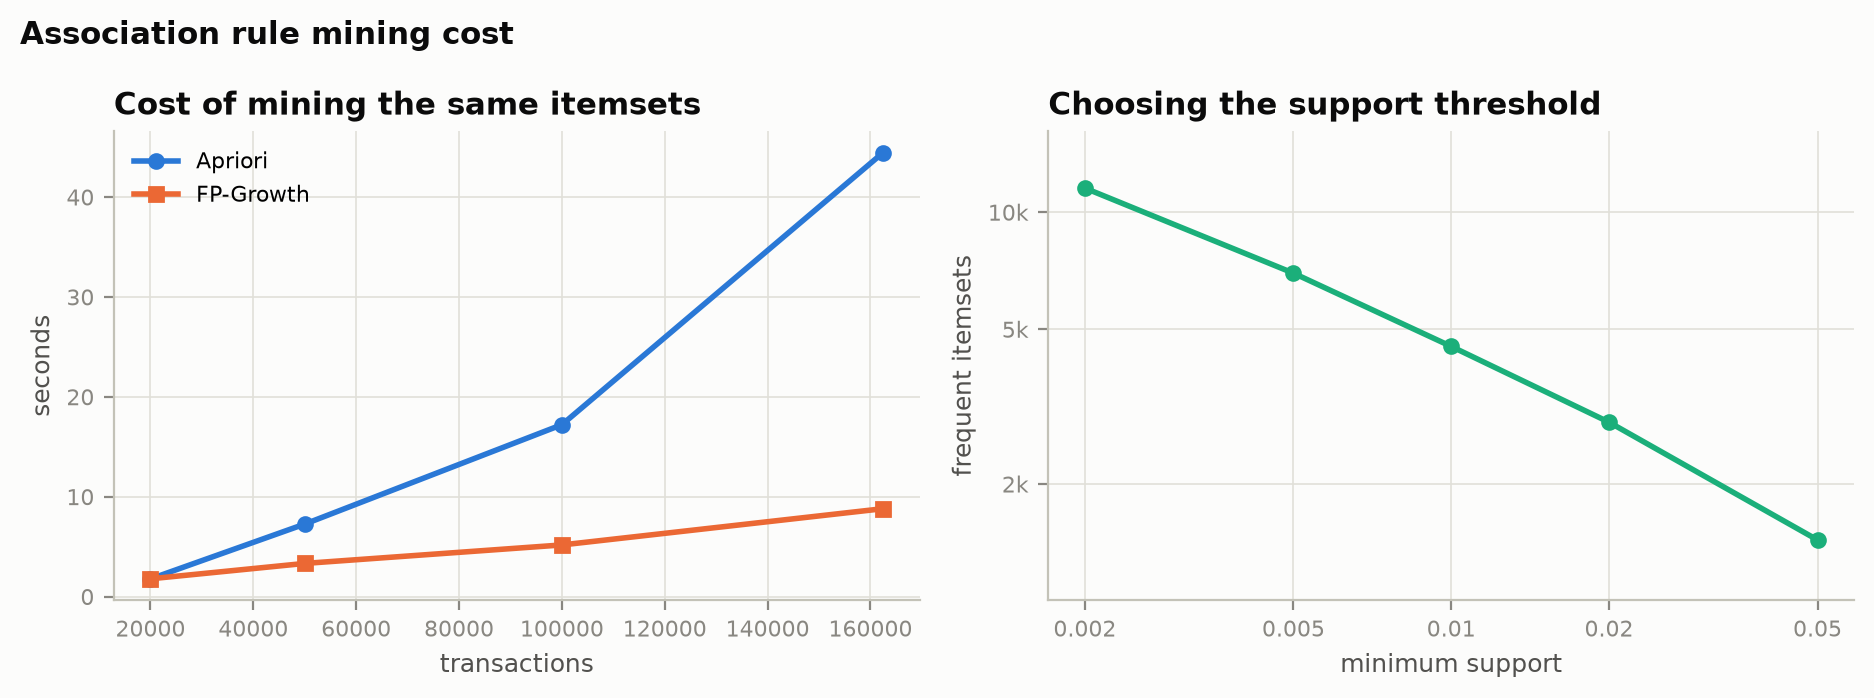
\includegraphics[width=0.92\linewidth]{03-rule-mining-cost.png}

  \smallskip
  \footnotesize
  Identical itemsets. Apriori rescans the database once per candidate level;
  FP-Growth builds its tree in two passes. \punch{At small $n$ Apriori is
  actually faster} --- the crossover is visible.
\end{frame}

% ---------------------------------------------------------------- accuracy
\begin{frame}{Accuracy is the wrong number}
  \centering
  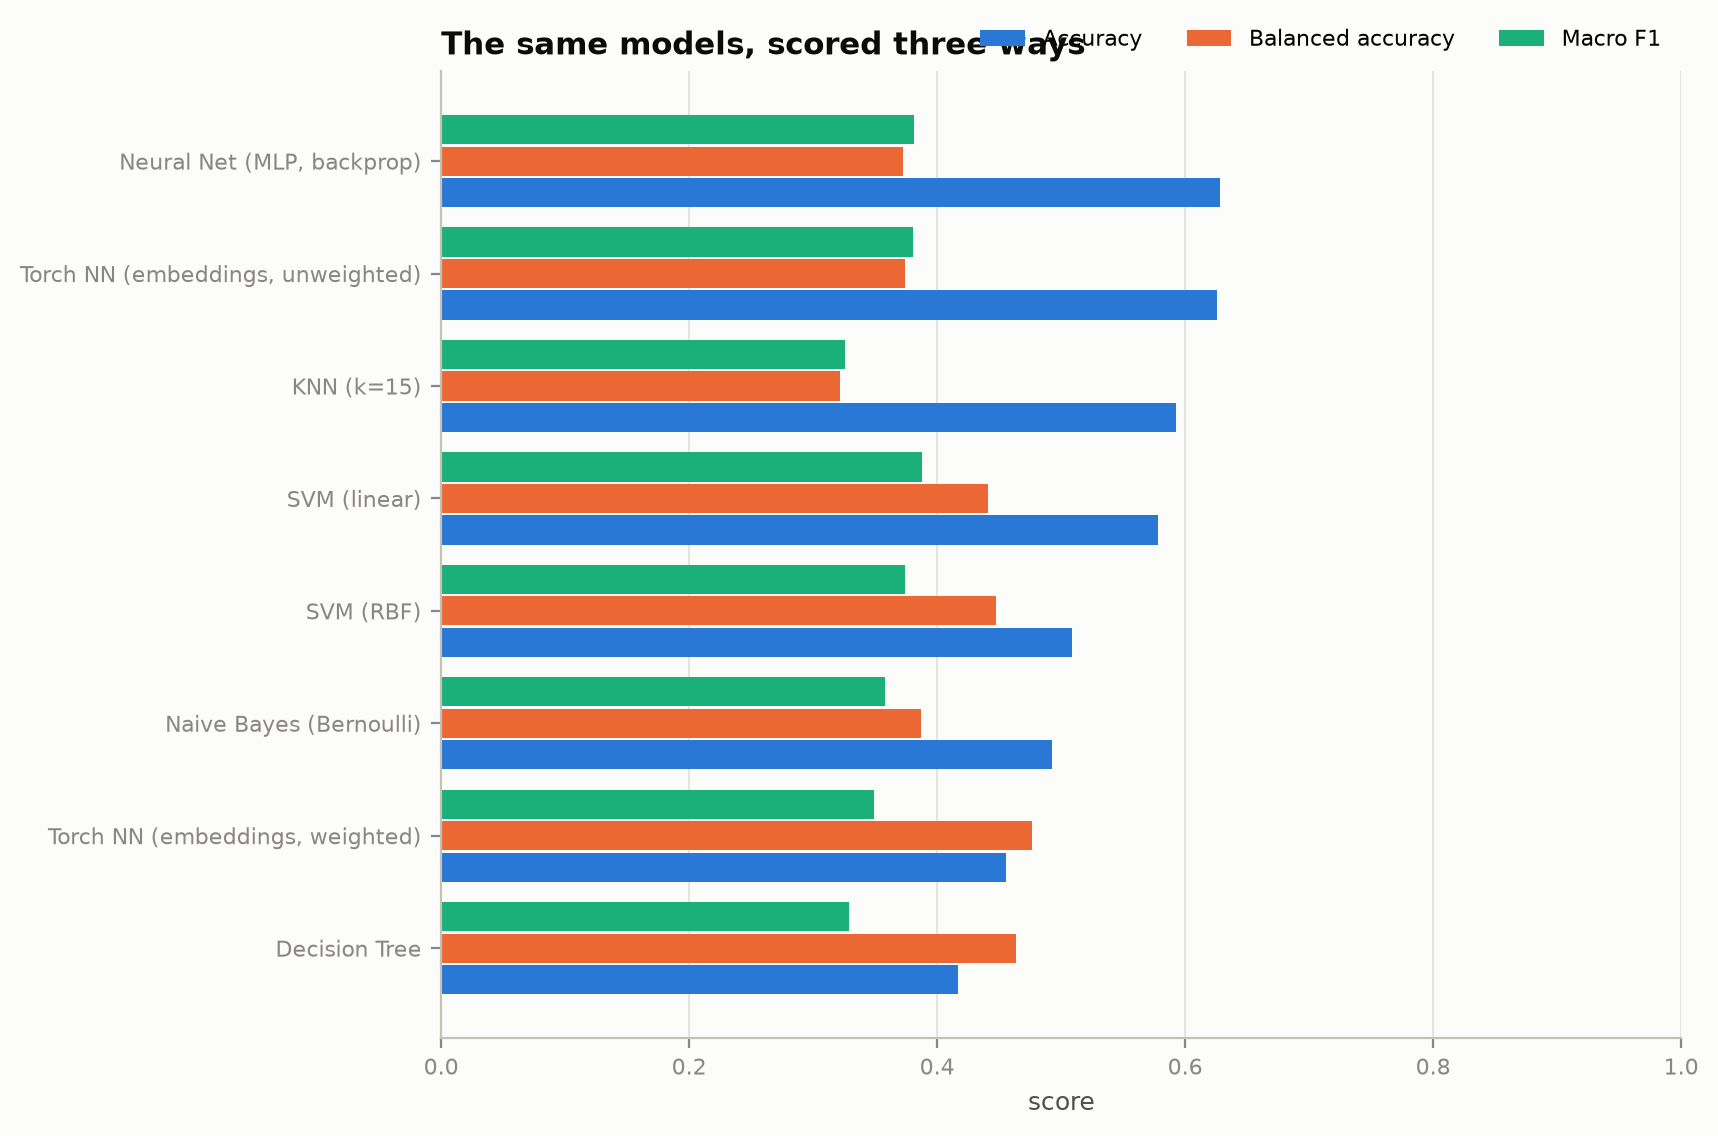
\includegraphics[height=0.68\textheight]{05-accuracy-trap.png}

  \footnotesize
  The models with the best accuracy have the worst balanced accuracy. They are
  predicting the majority class and being rewarded for it.
\end{frame}

\begin{frame}{Honest evaluation costs you accuracy you never had}
  \begin{columns}[T]
    \begin{column}{0.52\textwidth}
      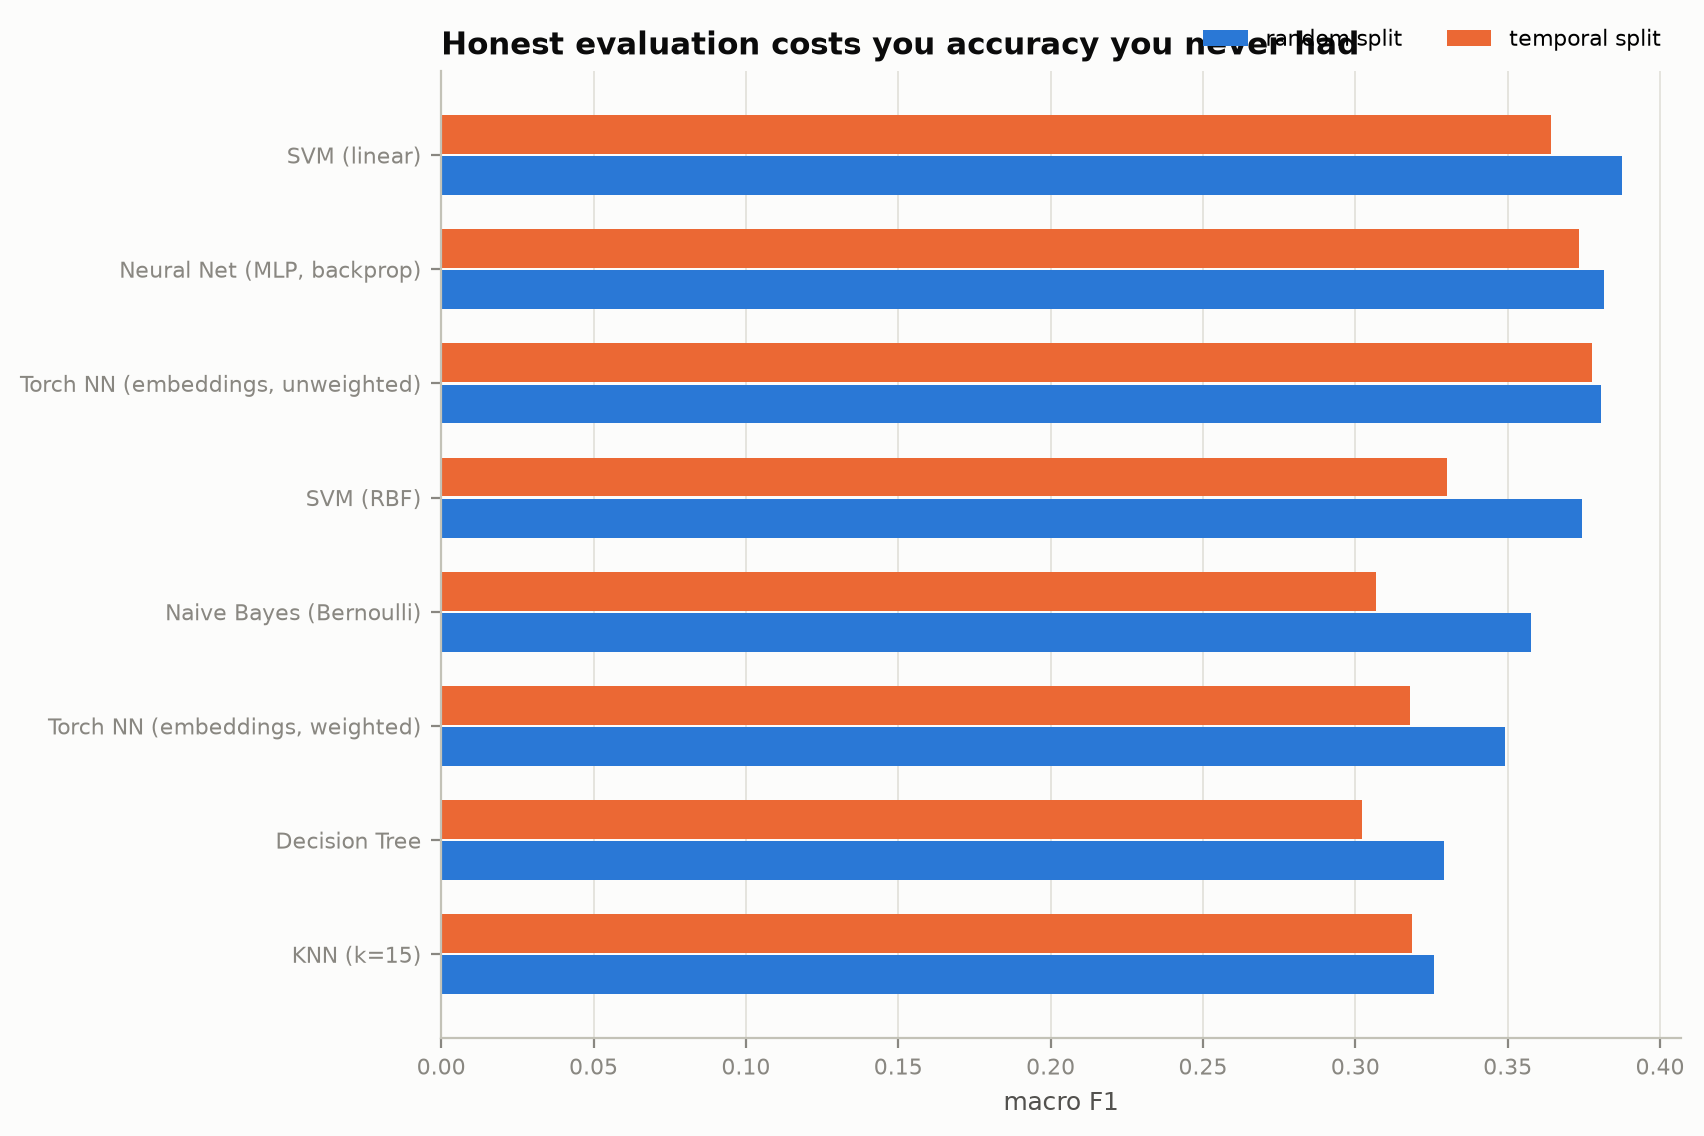
\includegraphics[width=\linewidth]{04-protocol-comparison.png}
    \end{column}
    \begin{column}{0.46\textwidth}
      \small
      A \textbf{random} split lets a model learn period-specific shelter policy
      and take credit for it.

      \smallskip
      Austin's intake collapsed from 19{,}775 in 2019 to 9{,}778 in 2020.

      \bigskip
      \punch{Train $\le$ 2021, test $\ge$ 2022.}
      \smallskip

      Every model degrades. No exceptions.
    \end{column}
  \end{columns}
\end{frame}

% ------------------------------------------------------------------- torch
\begin{frame}{We added a PyTorch network. Here is why it earns its place.}
  \small
  \texttt{MLPClassifier} is \emph{already} a backprop network. A second one needs
  a reason. There are two, and both are things scikit-learn cannot do:

  \medskip
  \begin{enumerate}\itemsep0.5em
    \item \punch{No \texttt{class\_weight} in \texttt{MLPClassifier}} --- which is
          exactly why it has the best accuracy (0.628) and nearly the worst
          balanced accuracy (0.373). It cannot resist the majority class.
    \item \punch{Learned embeddings} instead of one-hot. One-hot puts Labrador
          as far from Golden Retriever as from Siamese.
  \end{enumerate}

  \medskip
  \centering
  \begin{tabular}{@{}lrrr@{}}
    \toprule
    \textbf{Random split} & \textbf{accuracy} & \textbf{balanced acc.} & \textbf{macro F1} \\
    \midrule
    sklearn MLP (one-hot)     & 0.628 & 0.373 & 0.382 \\
    Torch, unweighted         & 0.626 & 0.374 & 0.381 \\
    Torch, weighted loss      & 0.455 & \textbf{0.477} & 0.349 \\
    \bottomrule
  \end{tabular}
\end{frame}

\begin{frame}{The weighting is a dial, and it has a price}
  \centering
  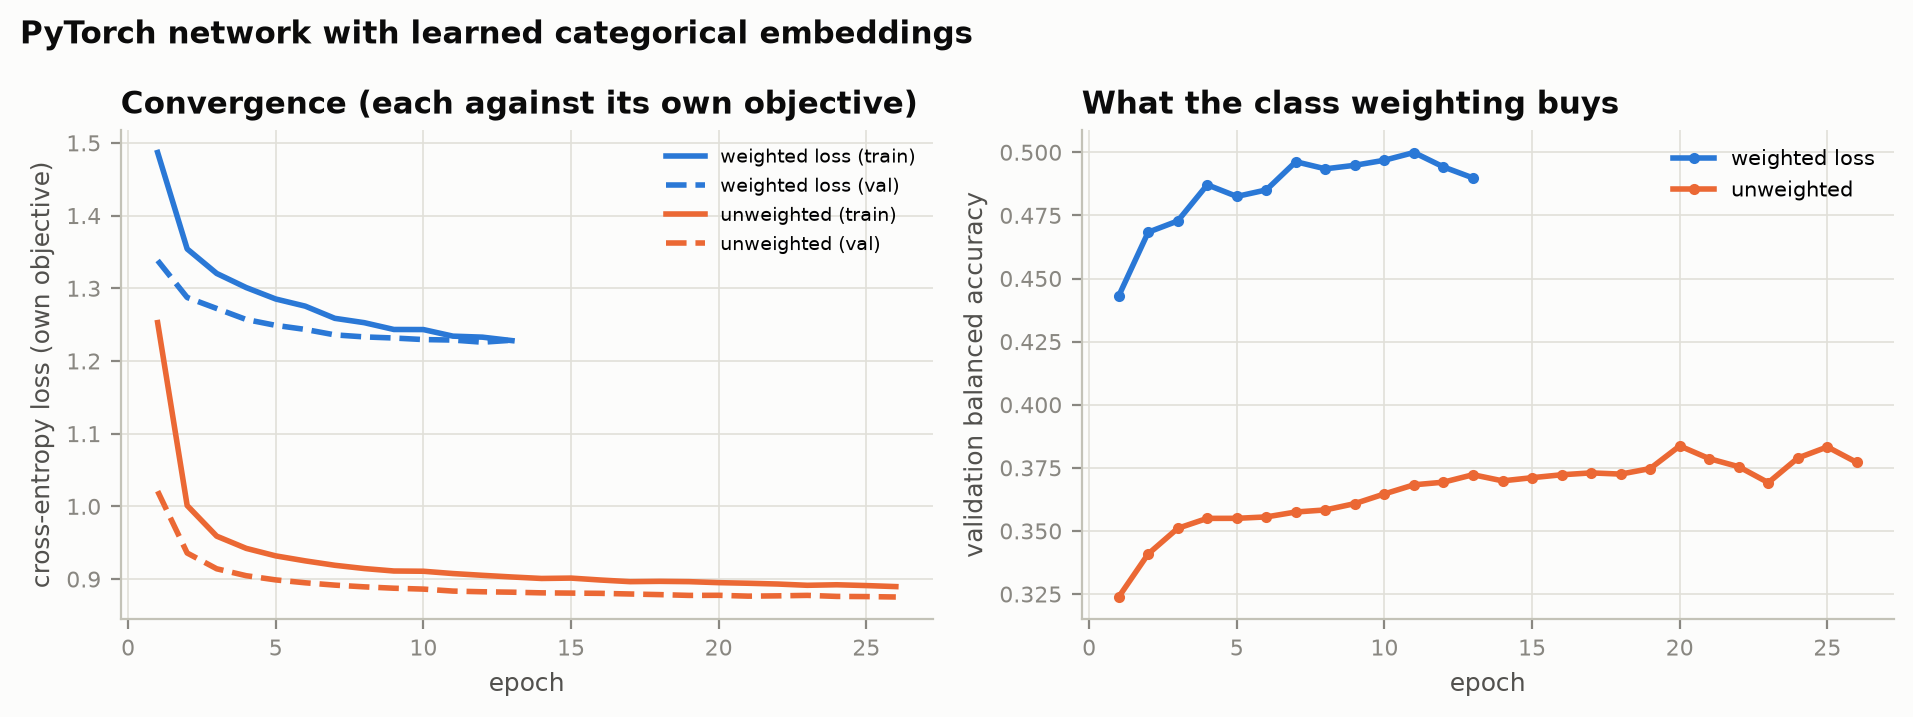
\includegraphics[width=0.95\linewidth]{13-torch-training.png}

  \smallskip
  \footnotesize
  Unweighted torch matches the sklearn MLP to within \textbf{0.003 on every
  metric} --- that near-identity is the \textbf{control}, and it says the
  embeddings alone buy nothing here. Weighting then buys $\sim$10 points of
  balanced accuracy and \punch{costs} macro F1 (0.381 $\rightarrow$ 0.349):
  over-predicting rare classes hurts their precision.
\end{frame}

% -------------------------------------------------------------- clustering
\begin{frame}{Why K-Means is in the comparison to lose}
  Every attribute is categorical, so Euclidean distance is meaningless.

  \bigskip
  \textbf{Hamming} --- the fraction of the 11 attributes on which two animals
  differ --- is the right measure. It takes only 12 values, which makes
  \texttt{eps} readable:

  \begin{center}
    \punch{\texttt{eps} $= 2/11$ \;$\equiv$\; ``animals differing in at most two
    attributes''}
  \end{center}

  \bigskip
  K-Medoids, Hierarchical, DBSCAN and OPTICS all accept a precomputed
  dissimilarity. \textbf{K-Means cannot} --- it computes means, and the mean of
  categorical vectors is not an animal.

  \bigskip
  A medoid is a real animal you can look up. A centroid is not.
\end{frame}

\begin{frame}{Headline: atypical animals fare worse}
  \centering
  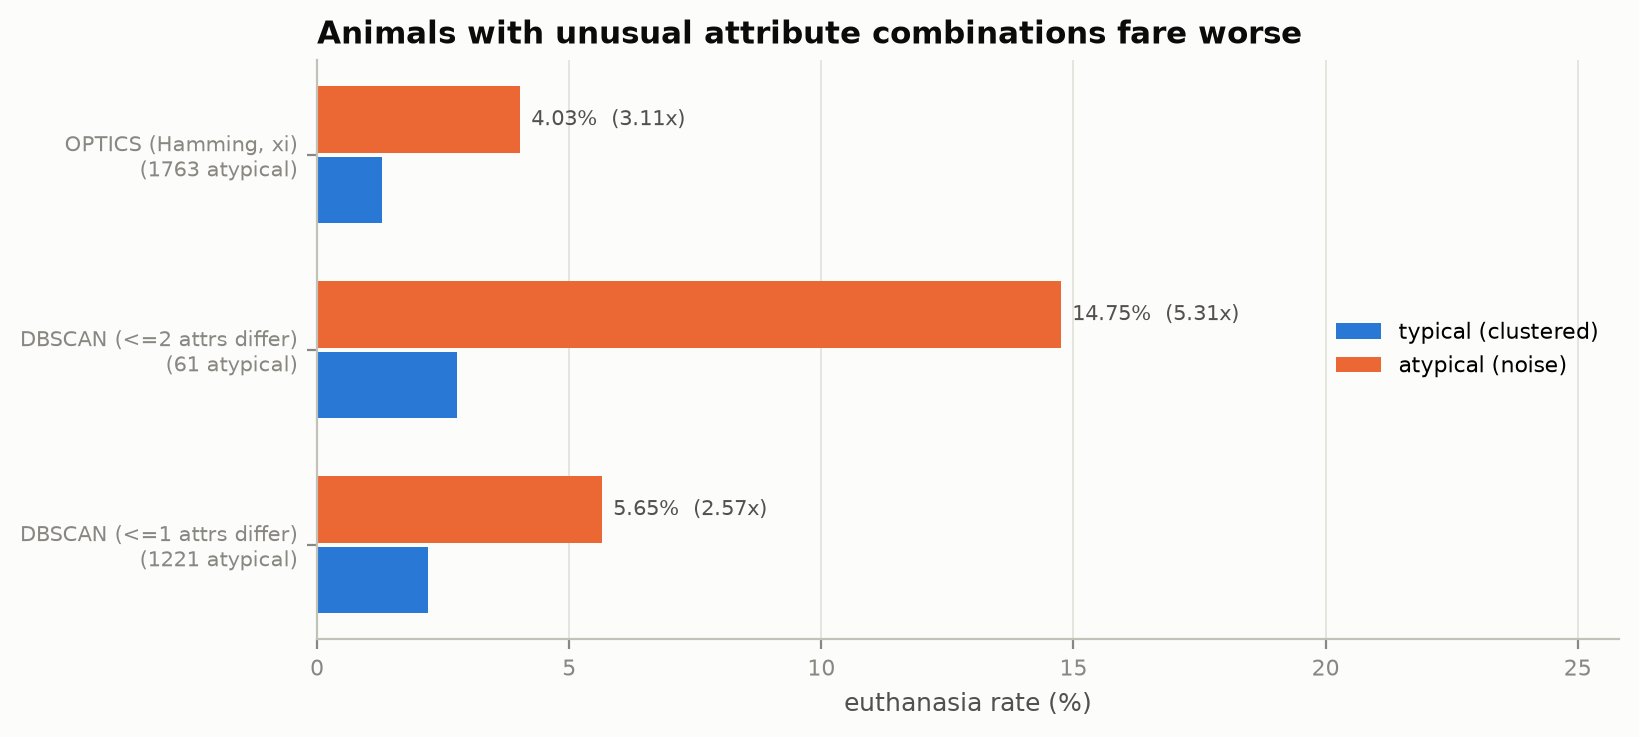
\includegraphics[height=0.66\textheight]{08-atypicality.png}

  \footnotesize
  Noise points are found with \textbf{no labels at all}. Labels only score the
  finding afterwards. Two density algorithms agree independently.
\end{frame}

% ------------------------------------------------------- rules versus tree
\begin{frame}{Two methods, same data, different attributes}
  \begin{columns}[T]
    \begin{column}{0.54\textwidth}
      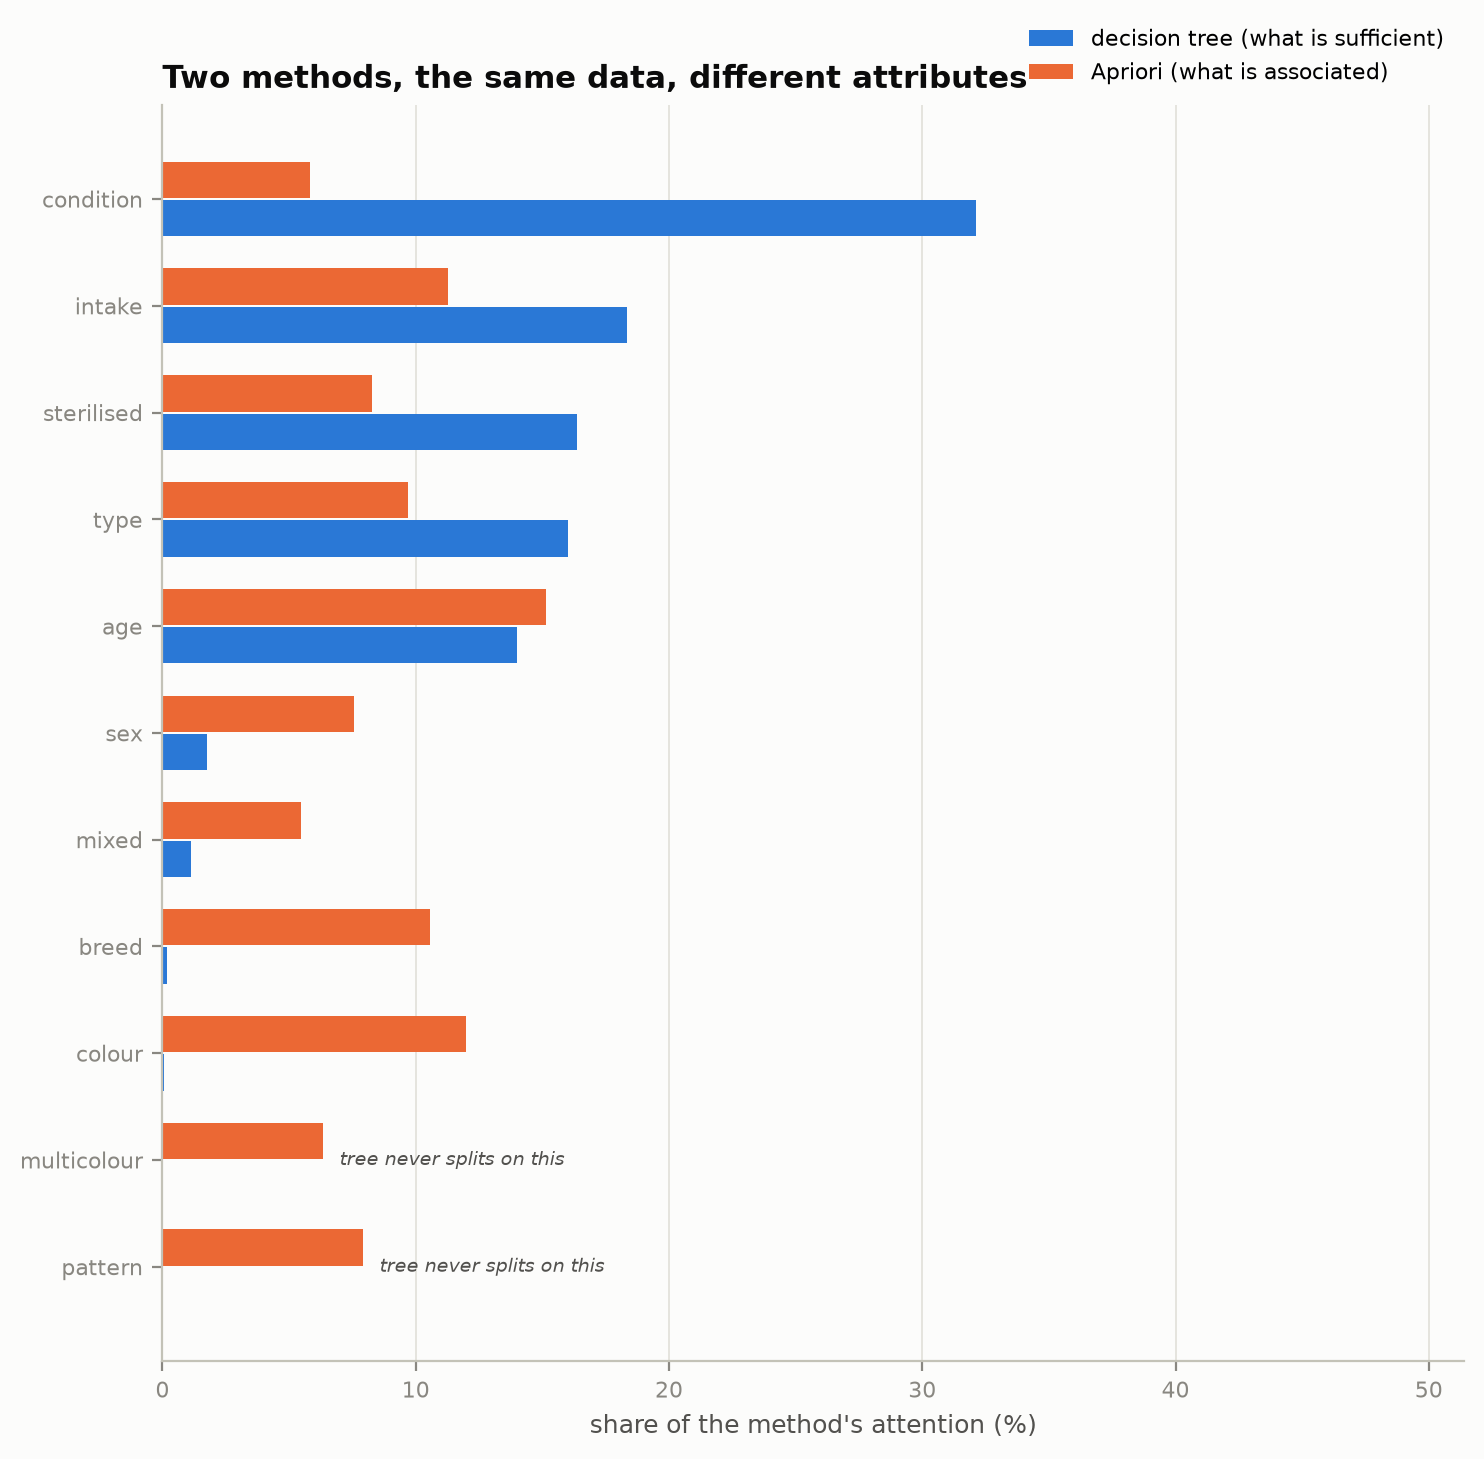
\includegraphics[width=\linewidth]{12-field-ranking.png}
    \end{column}
    \begin{column}{0.44\textwidth}
      \small
      Rank correlation $\approx$ \punch{zero}.

      \smallskip
      The tree \textbf{never splits on breed or colour}. Apriori reports both
      freely.

      \bigskip
      Not a contradiction --- two different questions:
      \begin{itemize}
        \item tree: what is \textbf{sufficient}
        \item Apriori: what is \textbf{associated}
      \end{itemize}

      \bigskip
      Yet $\sim$60\,\% of tree leaves \emph{do} have a matching mined rule.
    \end{column}
  \end{columns}
\end{frame}

% -------------------------------------------------------------------- bias
\begin{frame}{So: does colour decide an animal's fate?}
  \centering
  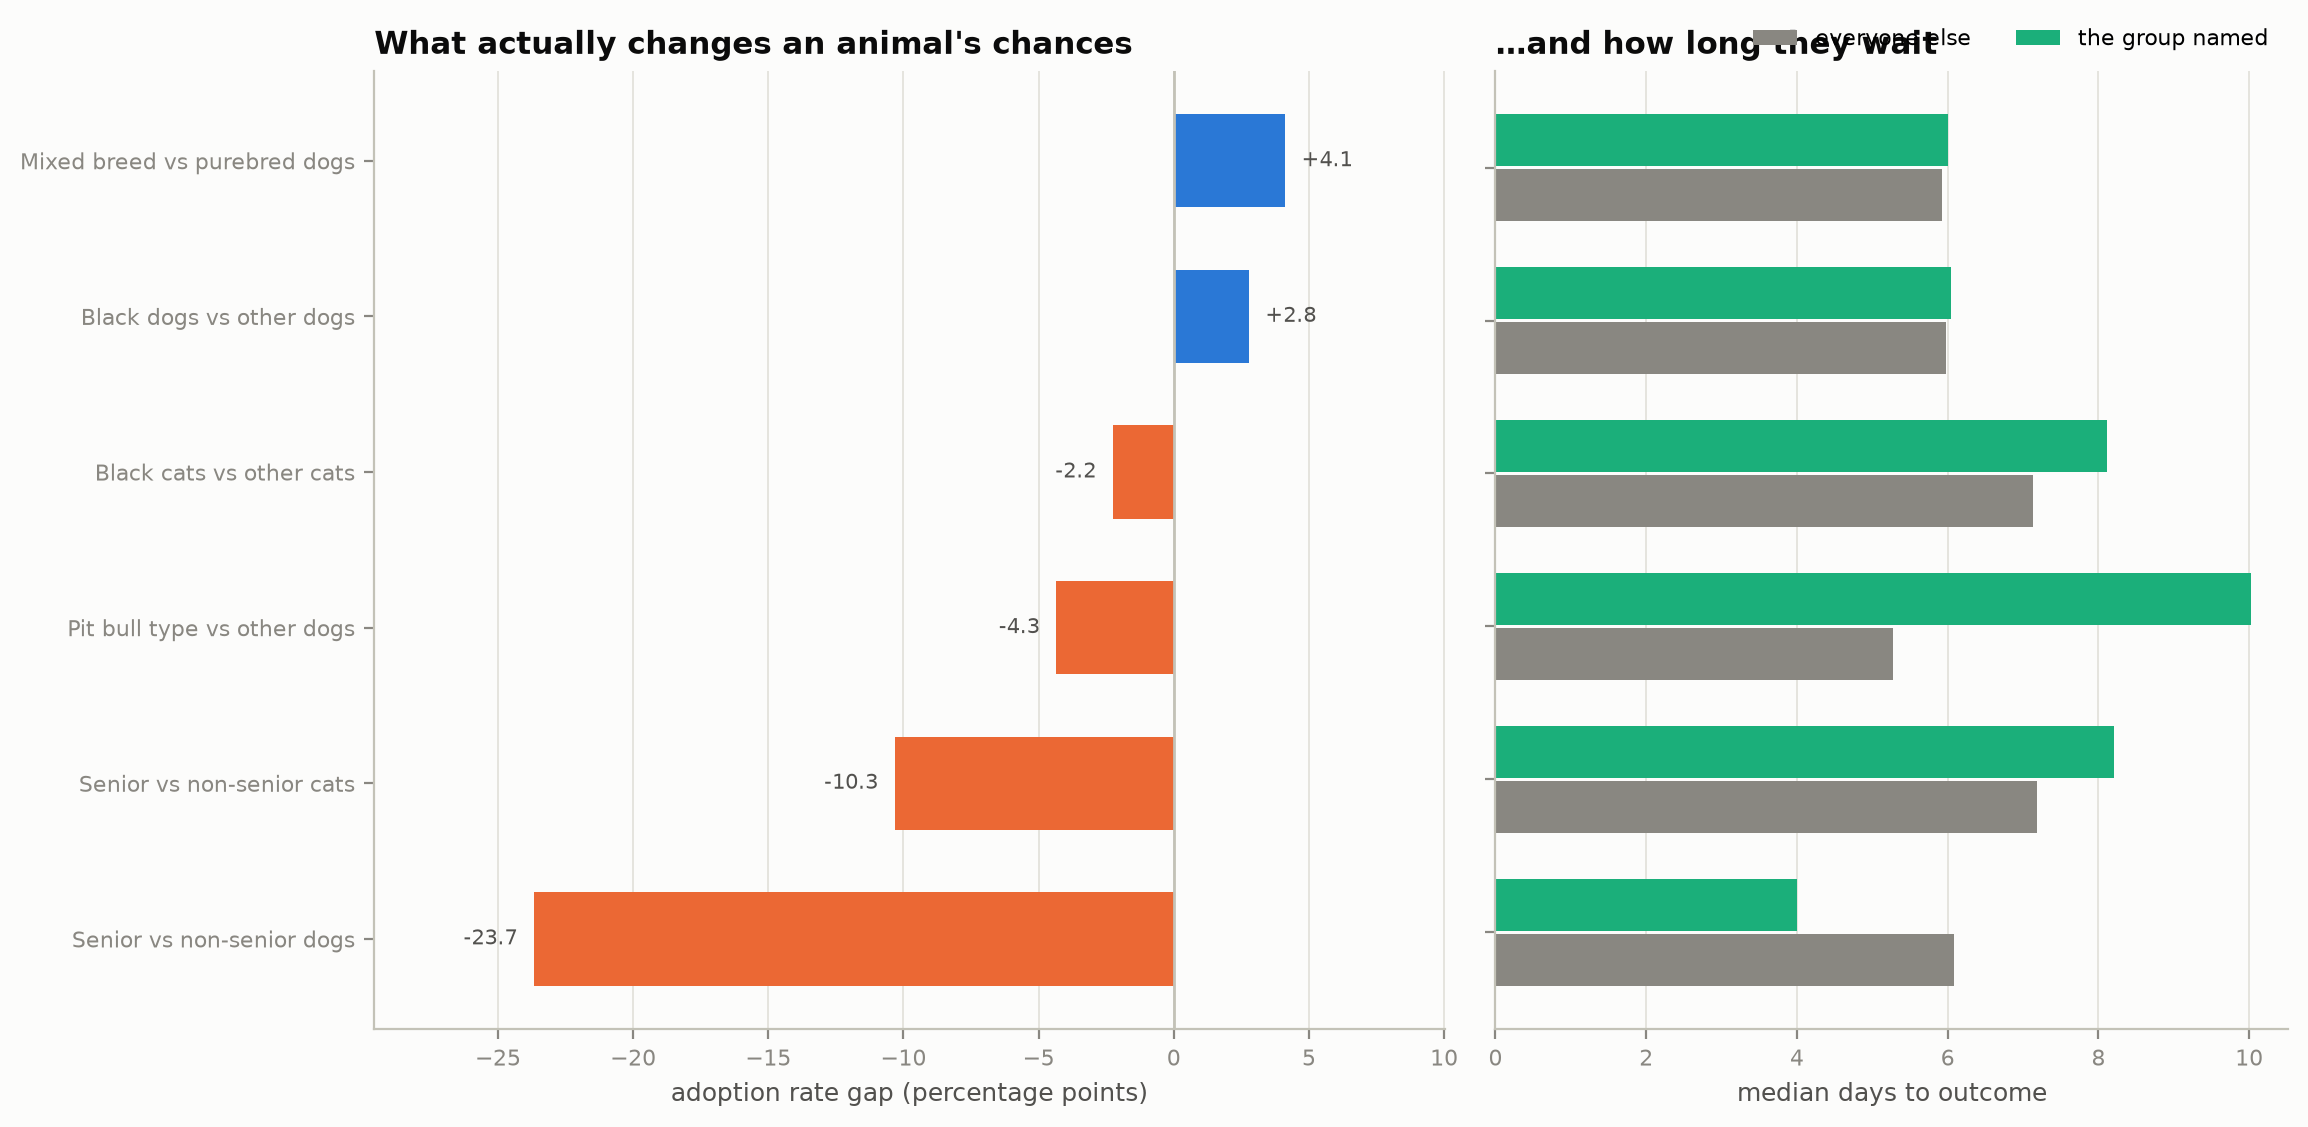
\includegraphics[width=0.95\linewidth]{10-claims.png}
\end{frame}

\begin{frame}{The answer}
  \Large
  \textbf{No.} Black dogs are adopted \punch{more} than other dogs.
  Black cats, 2.25 pp less --- about one extra day of waiting.

  \bigskip
  Standardised for species, age and intake route, \textbf{white} animals fare
  worst, not black ones.

  \bigskip\bigskip
  What actually decides it:
  \begin{itemize}\itemsep0.3em
    \item Senior dogs: \punch{$-$23.7 pp}
    \item Senior cats: $-$10.3 pp
    \item Pit bull type: $-$4.3 pp, and \punch{10.0 days' wait against 5.3}
  \end{itemize}

  \bigskip
  \normalsize The trait everyone argues about is nearly noise. The ones nobody
  mentions are large.
\end{frame}

% ------------------------------------------------------------- limitations
\begin{frame}{What we are not claiming}
  \begin{itemize}\itemsep0.7em
    \item \textbf{One shelter, one city.} Austin is a high-profile no-kill
          shelter; its euthanasia rate is not representative.
    \item \textbf{Clustering does not recover outcome classes} (ARI $\approx$
          0.02--0.04). Attribute clusters are not outcome clusters. We report
          this rather than tune it away.
    \item \textbf{Breed and colour are free text}, normalised by rules we wrote.
          98.9\,\% of records land in a named breed group; the mapping is
          published with the code.
    \item \textbf{Association, not causation.} Standardisation controls the
          confounders we measured, not the ones we did not.
    \item A guard marks any noise group below 30 animals unreliable --- one
          setting produced \textbf{three} noise points and a ``100\,\%
          euthanasia rate''.
  \end{itemize}
\end{frame}

% ------------------------------------------------------------------ closing
\begin{frame}{Conclusion}
  \begin{itemize}\itemsep0.7em
    \item The superstition is \textbf{measurably false}; age and breed label are
          \textbf{measurably large}.
    \item Density-based clustering finds animals at risk \textbf{without any
          labels} --- 2.7 to 3.2$\times$ the euthanasia rate.
    \item Rules and trees agree on \emph{rules} and disagree on \emph{attributes},
          and the disagreement explains the bias result by a third route.
    \item Honest temporal evaluation lowers every score. We report the lower one.
  \end{itemize}

  \bigskip
  \centering
  \punch{\large Every algorithm from the syllabus, doing real work.}

  \bigskip
  \footnotesize
  Code, tables and figures: \texttt{shelter/} --- one command reproduces everything.
\end{frame}

\begin{frame}[plain]
  \centering
  \vfill
  {\Huge\color{jiitblue}\textbf{Thank you}}
  \vfill
  \footnotesize Questions
  \vfill
\end{frame}

\end{document}
